%========================================================
\chapter{Detailed Design of the Proposed TBML Framework}
%========================================================

The detailed design of the proposed TBML detection framework focuses on the internal organization, analytical workflow, and module-level interaction associated with graph-based fraud detection and real-time financial monitoring. The framework integrates transaction processing services, heterogeneous graph construction, hybrid HGNN--LSTM analytical models, federated learning mechanisms, and compliance reporting modules within a unified monitoring environment. This chapter presents the structure chart, detailed module design, database schema organization, and monitoring workflow associated with the proposed TBML detection framework.

%========================================================
\section[Structure Chart]{\textbf{Structure Chart}}
%========================================================
The structure chart of the proposed TBML detection framework illustrates the hierarchical organization of the major functional modules operating within the system. The framework is divided into frontend, backend, fraud detection, federated learning, database, and compliance layers to support scalable financial monitoring and intelligent fraud analysis within distributed Anti-Money Laundering environments.

The frontend layer provides dashboard interfaces, transaction monitoring services, risk visualization, and STR management functionalities for institutional users. Backend services coordinate API communication, transaction processing, authentication workflows, and access control operations between frontend interfaces and analytical modules. The fraud detection layer incorporates Hybrid HGNN--LSTM components responsible for graph-based analysis, temporal transaction modeling, feature fusion, and risk classification.

The federated learning layer enables privacy-preserving collaborative model training and global model synchronization between participating institutions. Database services manage transactional storage, graph relationships, audit logs, and compliance-related records, while the compliance layer supports STR generation, regulatory reporting, email notifications, and monitoring operations. The overall structural organization of the proposed TBML detection framework is illustrated in Figure~\ref{fig:structure_chart}.
\begin{figure}[H]
    \centering
    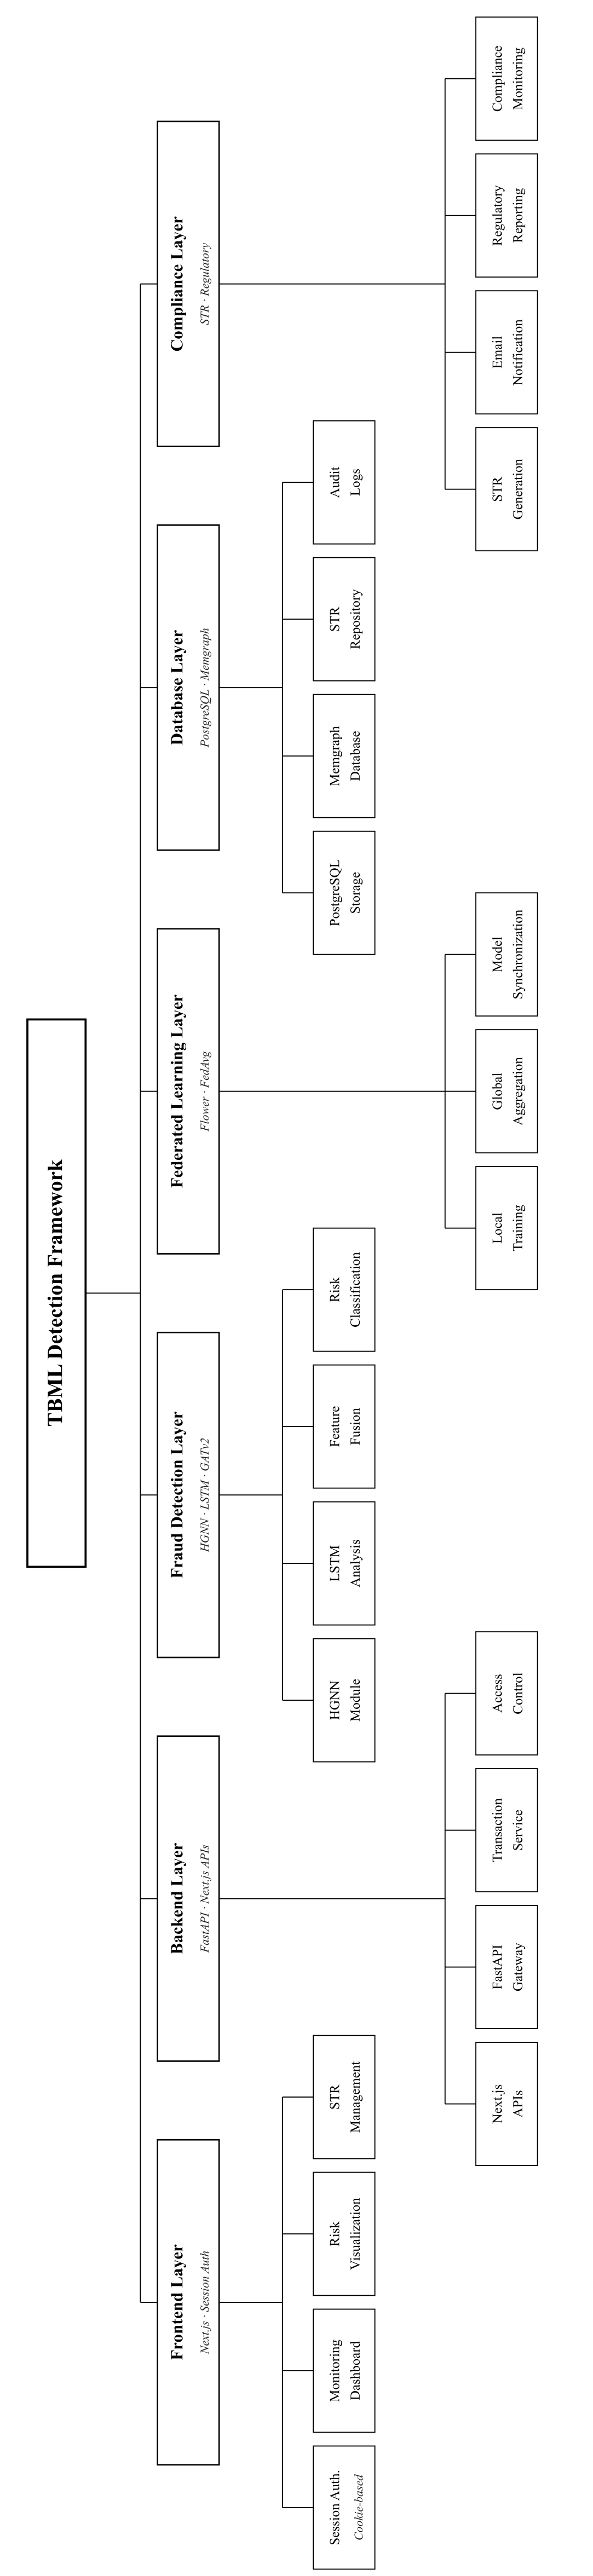
\includegraphics[height=0.95\textheight]{Figures/tbml_final_academic_structure_chart.png}
    \caption{Structure Chart of the Proposed TBML Detection Framework}
    \label{fig:structure_chart}
\end{figure}

The structure chart illustrates the modular organization and interaction between analytical, monitoring, storage, and compliance-oriented services within the proposed framework. This modular design approach improves scalability, maintainability, service integration, and efficient coordination between frontend interfaces, backend analytical services, and distributed fraud detection environments.

%========================================================
\section[Functional Description of the Modules]{\textbf{Functional Description of the Modules}}
%========================================================

The functional description of the modules explains the internal processing workflow and interaction between the major analytical, monitoring, and compliance-oriented components operating within the proposed TBML detection framework. The framework integrates transaction streaming services, graph construction mechanisms, hybrid HGNN--LSTM analytical models, institutional verification environments, and regulatory reporting systems to support intelligent Trade-Based Money Laundering detection and real-time compliance monitoring.

%========================================================
\subsection[Module Interaction Workflow]{\textbf{Module Interaction Workflow}}
%========================================================

The module interaction workflow illustrates the coordinated operational flow between transaction ingestion services, streaming environments, graph-based analytical modules, fraud classification mechanisms, institutional verification procedures, and regulatory monitoring systems functioning within the proposed framework. Financial transactions, KYC records, and trade documents are initially processed within the transaction processing layer and published into Kafka streaming topics for asynchronous event-driven communication between backend analytical services.

Kafka consumer services subsequently consume the transaction streams and forward the processed data to the graph construction and feature extraction module where heterogeneous financial transaction graphs are generated using accounts, transactions, trade entities, and document relationships stored within the Memgraph database. The extracted graph embeddings and relational features are processed by the Hybrid HGNN--LSTM fraud detection module to perform graph representation learning, temporal transaction analysis, and intelligent fraud prediction.

The generated fraud classifications and monitoring results are stored within the PostgreSQL database and visualized through the dashboard monitoring environment for institutional investigators and banking administrators. Suspicious transactions identified by the analytical system are reviewed by authorized bank administrators before being categorized as clean, suspicious, or confirmed fraudulent transactions.

Transactions verified as fraudulent are forwarded to the STR generation environment where Suspicious Transaction Reports are generated with analytical assistance from the Groq API service. Generated STR reports are subsequently reviewed by regulatory authorities responsible for investigation management, inquiry procedures, and enforcement operations. Notification management services coordinate fraud alerts and institutional communication processes, while the Resend email service delivers notification emails and regulatory enforcement messages to the corresponding institutional authorities. The overall module interaction workflow of the proposed TBML detection framework is illustrated in Figure~\ref{fig:workflow_interaction}.

\begin{figure}[H]
    \centering
    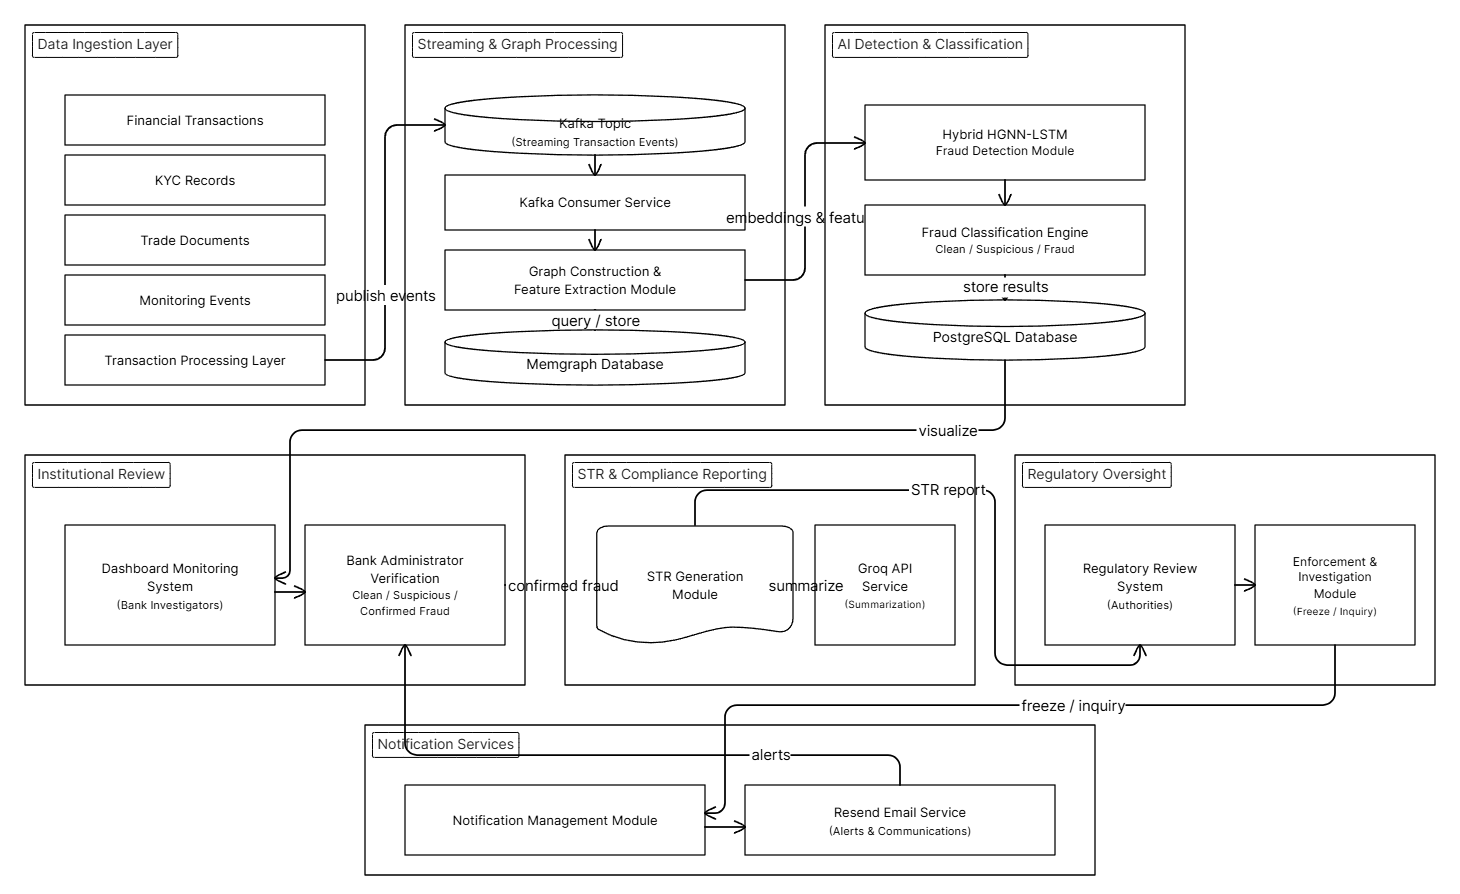
\includegraphics[width=\textwidth]{Figures/module-interaction2.png}
    \caption{Workflow Interaction Diagram for the Proposed TBML Detection Framework}
    \label{fig:workflow_interaction}
\end{figure}

The workflow interaction diagram illustrates the coordinated interaction between streaming services, graph-based analytical modules, monitoring environments, institutional verification systems, and regulatory compliance services operating within the proposed framework. Such modular workflow integration supports scalable transaction processing, intelligent fraud analysis, compliance management, and real-time Anti-Money Laundering monitoring within distributed financial environments.

%========================================================
\subsection[Transaction Processing Module]{\textbf{Transaction Processing Module}}
%========================================================

The transaction processing Module acts as the initial ingestion environment within the proposed TBML detection framework. This Module collects financial transactions, KYC records, trade documents, and institutional monitoring events originating from banking systems and external financial environments.

The input data processed within this Module includes sender and receiver account identifiers, transaction amounts, commodity types, trade quantities, trade values, invoice details, transaction timestamps, and institutional monitoring attributes associated with financial activities. The collected transactional data is validated, normalized, and converted into structured transaction records to support reliable downstream analytical processing.

The processed transaction events are published into Kafka streaming topics to enable asynchronous communication between backend services and analytical modules. The generated transaction streams serve as the primary input for graph construction, feature extraction, and graph-based fraud detection operations within the proposed framework.


%========================================================
\subsection[Graph Construction Module]{\textbf{Graph Construction Module}}
%========================================================

The graph construction module is responsible for transforming processed transaction streams into heterogeneous financial transaction graphs for graph-based analytical processing. This module receives validated transaction events from Kafka consumer services and models financial interactions between accounts, transactions, trade documents, and institutional entities within a connected graph environment.

The generated graph schema consists of interconnected node entities including \texttt{(:Account)}, \texttt{(:Transaction)}, and \texttt{(:Document)} connected through graph relationships such as \texttt{[:SENDS]}, \texttt{[:TO]}, and \texttt{[:HAS\_DOC]}. These relationships represent sender-receiver interactions, transaction ownership, trade associations, and document linkages required for identifying hidden transactional dependencies associated with Trade-Based Money Laundering activities.

The module interacts with the Memgraph database to store graph structures, entity relationships, and transactional connectivity information required for downstream analytical learning. The generated graph features and relational representations are subsequently forwarded to the Hybrid HGNN--LSTM fraud detection module for graph-based fraud analysis and intelligent transaction classification.

%========================================================
\subsection[Hybrid HGNN--LSTM Fraud Detection Module]{\textbf{Hybrid HGNN--LSTM Fraud Detection Module}}
%========================================================

The Hybrid HGNN--LSTM fraud detection module performs graph-based fraud analysis and temporal transaction modeling within the proposed TBML detection framework. The module receives KYC node features, transaction sequences, SWIFT edge attributes, and trade metadata generated from the graph construction environment for downstream analytical processing.

The graph branch utilizes multi-layer GATv2 operations to perform neighborhood aggregation and graph attention learning across interconnected financial entities. In parallel, the temporal branch utilizes LSTM-based sequential modeling to analyze transaction sequences and identify abnormal temporal transaction behavior associated with suspicious financial activities. The trade branch processes trade metadata and institutional transaction attributes using multilayer perceptron operations and feature normalization mechanisms.

The generated graph embeddings, temporal representations, and trade feature vectors are combined within the feature fusion layer for downstream fraud prediction and transaction risk analysis. The dense classification layer categorizes transactions into predefined classes including \texttt{CLEAN}, \texttt{WATCHLIST}, and \texttt{FRAUD}. The overall architecture of the proposed Hybrid HGNN--LSTM fraud detection module is illustrated in Figure~\ref{fig:hgnn_architecture}.

\begin{figure}[H]
    \centering
    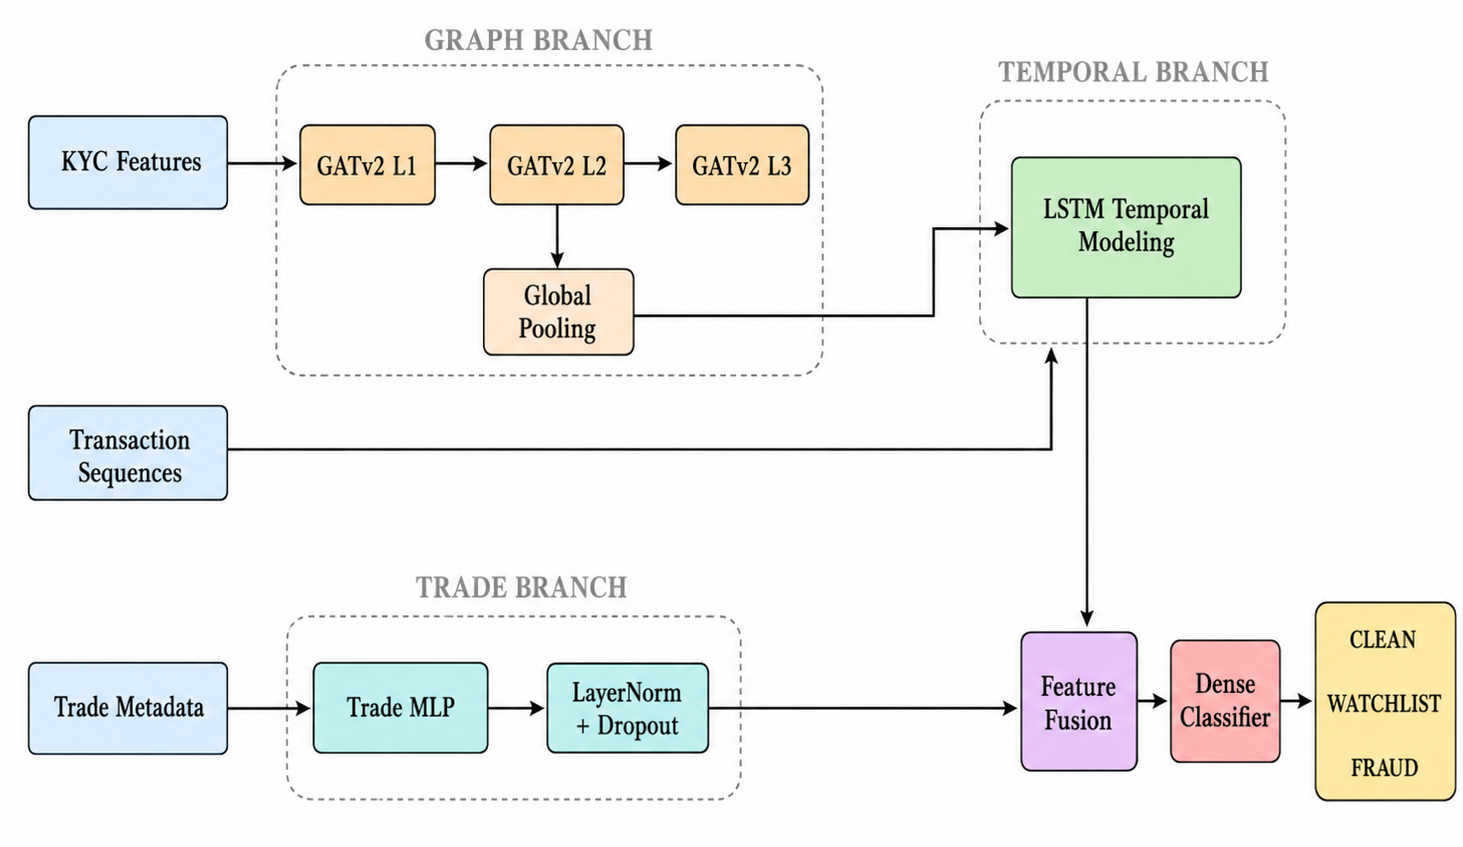
\includegraphics[width=\textwidth]{Figures/aimodel.png}
    \caption{Architecture of the Proposed Hybrid HGNN--LSTM Fraud Detection Module}
    \label{fig:hgnn_architecture}
\end{figure}



%========================================================
\subsection[Federated Learning Module]{\textbf{Federated Learning Module}}
%========================================================

The federated learning module enables privacy-preserving collaborative fraud detection across distributed financial institutions without directly sharing sensitive transactional data. Each participating institution performs local model training using institutional transaction graphs, transaction sequences, and fraud classification labels generated within the analytical environment.

The locally trained model parameters are periodically transmitted to the central aggregation server where the Federated Averaging (\texttt{FedAvg}) strategy combines local model updates to generate an optimized global fraud detection model. The aggregated global model is subsequently redistributed to participating institutions for continuous fraud detection and real-time analytical inference. The overall federated learning architecture of the proposed framework is illustrated in Figure~\ref{fig:federated_architecture}.

\begin{figure}[H]
    \centering
    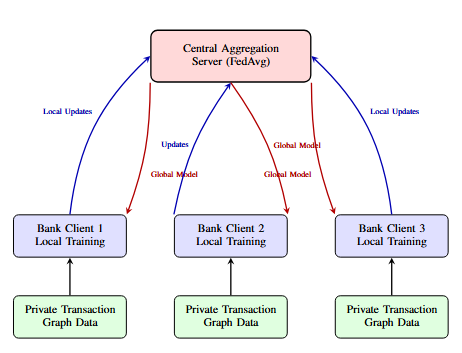
\includegraphics[width=0.82\textwidth]{Figures/federated_architecture.png}
    \caption{Federated learning architecture for privacy-preserving collaborative TBML detection across distributed institutions}
    \label{fig:federated_architecture}
\end{figure}



%========================================================
\subsubsection[STR Generation and Notification Module]{\textbf{STR Generation and Notification Module}}
%========================================================

The STR generation and notification module is responsible for compliance reporting and fraud alert management within the proposed TBML detection framework. Transactions verified as fraudulent by authorized banking administrators are forwarded to this module for Suspicious Transaction Report (STR) generation and regulatory processing. The module generates STR reports containing transaction details, fraud classifications, trade metadata, institutional information, and investigation summaries associated with suspicious financial activities.

The Groq API service is utilized for analytical summarization and automated assistance during compliance documentation generation. Generated STR reports are subsequently forwarded to regulatory monitoring authorities for investigation and enforcement procedures. The notification management environment coordinates fraud alerts and institutional communication workflows, while the Resend email service delivers notification emails, investigation alerts, and regulatory enforcement messages to banking institutions and regulatory authorities.
%========================================================
\subsubsection[Dashboard and Regulatory Monitoring Module]{\textbf{Dashboard and Regulatory Monitoring Module}}
%========================================================

The dashboard and regulatory monitoring module provides real-time transaction visualization, fraud monitoring, and institutional investigation functionalities within the proposed TBML detection framework. The monitoring dashboard displays transaction classifications, fraud alerts, risk scores, STR records, and analytical monitoring information generated by the fraud detection environment. Separate dashboard environments are maintained for banking administrators and regulatory authorities to support institution-level monitoring and centralized compliance management operations.

Authorized banking administrators can view suspicious and fraudulent transactions identified by the analytical model and perform institutional verification procedures before categorizing transactions as \texttt{CLEAN}, \texttt{WATCHLIST}, or \texttt{FRAUD}. Suspicious transactions can either be escalated as fraudulent transactions or marked as clean after institutional verification procedures, thereby reducing false positive classifications within the monitoring environment. Transactions verified as fraudulent are subsequently forwarded for Suspicious Transaction Report (STR) generation and regulatory reporting.

Regulatory authorities monitor generated STR reports and institution-level fraud cases through centralized monitoring dashboards. The regulatory environment supports compliance monitoring, document verification requests, inquiry procedures, and account freeze operations associated with suspicious financial activities.




% %========================================================
% \section[Sequence Diagram for TBML Detection Workflow]{\textbf{Sequence Diagram for TBML Detection Workflow}}
% %========================================================

% The sequence diagram illustrates the dynamic interaction between the major system components involved in transaction monitoring, graph-based fraud analysis, federated learning, and compliance alert generation within the proposed TBML detection framework. The workflow begins when the monitoring dashboard initiates a transaction monitoring request through the banking environment. Transaction events are streamed and forwarded to the graph construction module where heterogeneous graph structures and analytical features are generated for fraud analysis.

% The generated graph data is processed by the Hybrid HGNN--LSTM analytical model to perform graph representation learning and temporal transaction analysis. Local model updates generated during training are transmitted to the federated learning server where global aggregation and model synchronization are performed using federated averaging mechanisms. The updated global model is subsequently utilized by the detection engine to perform fraud inference, generate risk classifications, and identify suspicious transactional behavior.

% Once suspicious activity is detected, the STR and notification service generates compliance reports and triggers alert notifications for institutional monitoring environments. The overall interaction flow between the major components of the proposed TBML detection framework is illustrated in Figure~\ref{fig:sequence_diagram}.

% \begin{figure}[H]
%     \centering
%     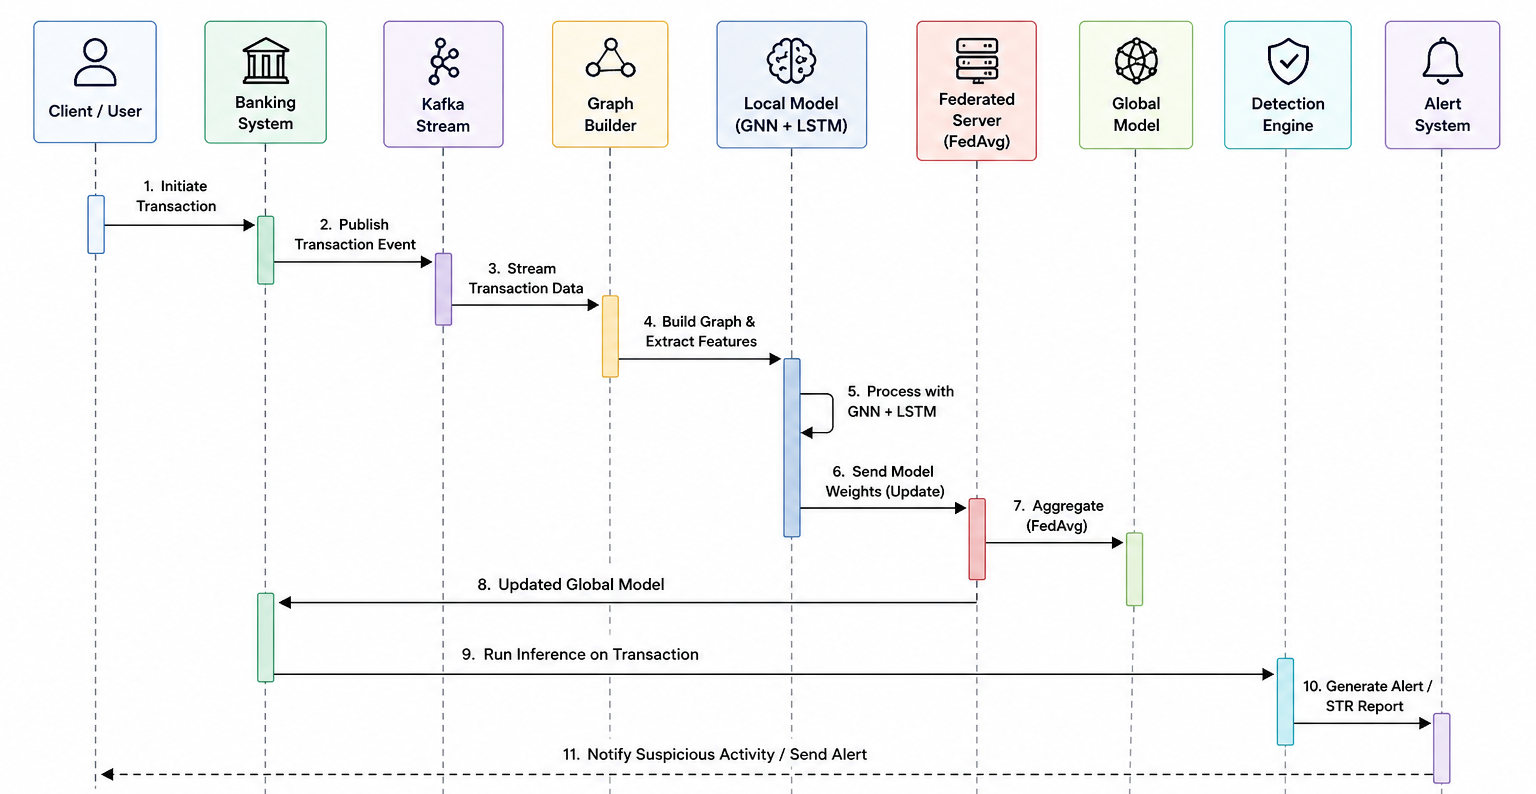
\includegraphics[width=\textwidth]{Figures/sequencediagramfinal.png}
%     \caption{Sequence Diagram for TBML Detection Workflow}
%     \label{fig:sequence_diagram}
% \end{figure}

% The sequence diagram demonstrates the coordinated interaction between frontend interfaces, transaction streaming services, analytical modules, federated learning environments, and compliance reporting systems operating within the proposed framework. Such coordinated workflows enable scalable real-time fraud detection, privacy-preserving collaborative learning, and efficient Anti-Money Laundering monitoring operations.
% %========================================================
% \section[Database Schema Design]{\textbf{Database Schema Design}}
% %========================================================



%========================================================
\section[Summary]{\textbf{Summary}}
%========================================================

This chapter presented the detailed design of the proposed TBML detection framework including the structural organization, module interaction workflow, functional description of analytical modules, federated learning architecture, and database management environment associated with the system. The chapter discussed the interaction between transaction processing services, graph construction mechanisms, hybrid HGNN--LSTM analytical modules, dashboard monitoring environments, and compliance reporting systems operating within the proposed framework.

The detailed design further illustrated how streaming-based transaction processing, graph-based fraud analysis, federated collaborative learning, institutional verification, STR generation, and regulatory monitoring are integrated within a unified Anti-Money Laundering environment. The subsequent chapter discusses the implementation details, backend integration and dashboard development associated with the proposed TBML detection framework.